\section{ЗАДАНИЕ}

Используя  базу знаний, хранящую знания (лаб. 13):

\begin{itemize}
    \item <<Телефонный справочник>>: Фамилия, №тел, Адрес – структура (Город, Улица, №дома, №кв),
    \item <<Автомобили>>: Фамилия\_владельца, Марка, Цвет, Стоимость, и др.,
    \item <<Вкладчики банков>>: Фамилия, Банк, счет, сумма, др.
\end{itemize}

Владелец может иметь несколько телефонов, автомобилей, вкладов (Факты). В разных городах есть однофамильцы, в одном городе – фамилия уникальна.

Используя конъюнктивное правило и простой вопрос, обеспечить возможность поиска:

По Марке и Цвету автомобиля найти Фамилию, Город, Телефон и Банки, в которых владелец автомобиля имеет вклады. Лишней информации не находить и не передавать!!!

Владельцев может быть несколько (не более 3-х), один и ни одного.

\begin{lstlisting}[caption=Текст программы]
domains
	lastname, phonenumber = string.

	city, street = string.
	house, flat = integer.
	address = address(city, street, house, flat).

	mark, color = string.
	cost = integer.

	bank, bankaccount = string.
	sum = integer.

predicates
	telephone(lastname, phonenumber, address).
	car(lastname, mark, color, cost, city).
	deposit(lastname, bank, bankaccount, sum, city).
	findWithCar(mark, color, lastname, city, phonenumber, bank).

clauses
	telephone("Ivanov", "123456", address("Moscow", "Pyshkinskaya", 12, 13)).
	telephone("Ivanova", "123421", address("Moscow", "Pyshkinskaya", 12, 13)).
	telephone("Ivanov", "654321",
		address("Saint-Petersburg", "Sadovaya", 10, 127)).
	telephone("Ivanov", "222444",
		address("Saint-Petersburg", "Sadovaya", 10, 127)).
	telephone("Petrov", "554322", address("Moscow", "Baymanskaya", 7, 53)).
	telephone("Petrov", "223544", address("Moscow", "Baymanskaya", 7, 53)).

	car("Ivanov", "Mercedes", "Black", 3000000, "Moscow").
	car("Ivanova", "Mercedes", "Black", 3000000, "Moscow").
	car("Ivanov", "Renault", "Gray", 1200000, "Moscow").
	car("Ivanov", "Lamborghini", "Yellow", 6000000, "Saint-Petersburg").
	car("Petrov", "Audi", "Red", 2000000, "Moscow").
	car("Petrov", "Infiniti", "Black", 4000000, "Moscow").

	deposit("Ivanov", "Tinkoff", "111222333444", 40000, "Moscow").
	deposit("Ivanova", "Tinkoff", "117227337447", 20000, "Moscow").
	deposit("Ivanov", "Sberbank", "444333222111", 100000, "Moscow").
	deposit("Ivanov", "Tinkoff", "123456789000", 150000, "Saint-Petersburg").
	deposit("Petrov", "Alpha-bank", "222333111444", 10000, "Moscow").
	deposit("Petrov", "Sberbank", "123123321321", 120000, "Moscow").

	findWithCar(Mark, Color, Lastname, City, Phonenumber, Bank) :-
		car(Lastname, Mark, Color, _, City),
		telephone(Lastname, Phonenumber, address(City, _, _, _)),
		deposit(Lastname, Bank, _, _, City).

goal
	%findWithCar("Mercedes", "Black", Lastname, City, Phonenumber, Bank).
	%findWithCar("Lamborghini", "Yellow", Lastname, City, Phonenumber, Bank).
	findWithCar("Infiniti", "Red", Lastname, City, Phonenumber, Bank).
\end{lstlisting}

\section{РЕЗУЛЬТАТЫ РАБОТЫ}

\begin{figure}[H]
    \centering
    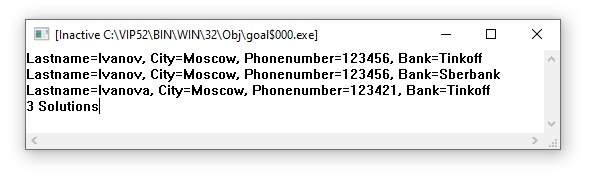
\includegraphics[scale=0.8]{img/1.jpg}
    \caption{findWithCar(``Mercedes'', ``Black'', Lastname, City, Phonenumber, Bank).}
\end{figure}

\begin{figure}[H]
    \centering
    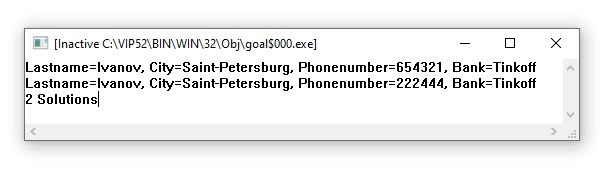
\includegraphics[scale=0.8]{img/2.jpg}
    \caption{findWithCar(``Lamborghini'', ``Yellow'', Lastname, City, Phonenumber, Bank).}
\end{figure}

\begin{figure}[H]
    \centering
    
\includegraphics[scale=0.8]{img/3.jpg}
    \caption{findWithCar(``Infiniti'', ``Red"'', Lastname, City, Phonenumber, Bank).}
\end{figure}
